\chapter{Discussion}
\label{sec:Discussion}
\section{Review of Results}
% Overview of results
%% Parameters under-constrained
%% Output estimates good
The results unequivocally show that the parameters of the BOLD model are under
constrained. While unsurprising given the sensitivity analysis in \cite{Deneux2006},
it is still an important limitation when calculating parameters. Thus, other methods
that depend on a point estimate of the parameters, such as least squares 
or kalman filters (which uses the first two moments) are limited. While estimates of
the  BOLD signal may still be correct, the estimate
of the underlying parameters and state variables are suspect. Similarly, as the
histograms in \autoref{sec:Multi-voxel Simulation} and \autoref{sec:Real Data Parameter Estimates}
show, using the mean to estimate parameters also makes little sense in the particle filter
case. Attributing the variance of estimate to the underlying parameter distribution would
also be a mistake; given that variance persisted even in simulated data. While parameters 
definitely vary from person to person and cortex to cortex, the estimated distributions 
in \autoref{sec:Real Data Parameter Estimates} are wider than the true underlying 
distribution. For this reason and because of the nonlinear relation between
parameters, any analysis should take the entire posterior estimate into account, 
rather than relying on an idealized Gaussian. In this sense, particle filters represent
an important step forward in BOLD parameter estimation. Representing
the uncertainty in parameters as a Gaussian is insufficient; so using a particle filter
or Bayesian estimate of the posterior is not simply an enhancement, but a necessary precaution.

Although point estimates of parameters are not dependable estimates of the 
true parameters, they still useful. Analysis of differences in parameters
could be medically relevant for instance. Additionally, a single estimate for parameters is still able
to form an accurate estimate of the BOLD signal. This trait bridges the gap with earlier types 
of activation tests, such as the statistical
parametric mapping. As the results in \autoref{sec:RealData} show, the heatmaps, especially
those of mutual information, closely resembled the results of SPM. While the activation
tests were more sensitive, there were some false positive, though at this point it is
difficult to quantify. It is
worth noting that certain enhancements could be useful in reducing false positives; for instance
by using the maximum likelihood, or median of the final distribution.  Future work may 
shed further light on these techniques. 

% Pros/Cons
%% Cons
%%% Computation longer than SPM
%%% Harder to interpret
%% Pro
%%% Non-parametric
%%% Real time
%%% Full Posterior
%%% More intuitive
\section{Particle Filter Review}
The Particle Filter algorithm was originally designed for on-line parameter 
estimation. For this reason, there is no guarantee of optimality or even 
convergence for finite measurements. However, for the BOLD nonlinear ODE 
this is less of a concern than it might first appear to be. For this
particular problem there can be no guarantee of a global minimum, and although
other techniques guarantee a local minimum, the particle filter doesn't settle 
to one of these local minima because it can settle into multiple ones. This
difference typifies the major difference between the particle filter and 
competing approaches. 

One difficulty
with the use of a particle filter with a finite number of datapoint is the calculation of a good
weight function $P(y_k | x_k)$  that will converge reasonably quickly. If the weight
function does not sufficiently differentiate particles, the final distribution will 
no be significantly different from the prior distribution. On the other hand, if the 
weight function is too thin, it will unfairly eliminate viable particles. Given sufficient
measurements it is better to let the algorithm take longer to converge, because the
convergence will be better (more accurate). The particle filter takes longer
to run than Volterra approximation method from \autoref{sec:Background Linear Approximation};
however, it is free from the uncertainty of whether a quadratic approximation is 
sufficient for the BOLD model. 

The particle filter certainly has significant advantages over other estimation procedures
discussed in \autoref{sec:Prior Works}. The most important advantage is that it provides
an estimate of the posterior probability, rather than a single estimate. While it is natural
to want a simple estimate of parameters, such an estimate is impossible with this particular
model. The results are more difficult to interpret, but this is a necessity. The fact that 
the final distribution is not dependent on any particular distribution is also advantageous.
Of particular note; the final distribution does not need to conform to any parametric
distribution. While the particle filter was not fast for full brain calculations, its speed
was sufficient on a quad core machine to perform real time calculations of small regions
(approximate run time .27 seconds per voxel-measurement). Today it would be possible
 to perform real time analysis of 10 voxels on an average quad core. The algorithm also scales
well and does not require burdensome amounts of memory (approximately 11 megabytes). 
For this reason this algorithm is perfect for extension to vector or video card
based processors. 

A more practical benefit with the particle filter is that it is mathematically
simple. An understanding of Bayesian statistics is all that is necessary to understand
how the particle filter works. This is in contrast to the Volterra based approach
of \cite{Friston2000}, which is quite complex. Additionally very few assumptions
are needed for the particle filter. It is a common problem in traditional statistics 
for assumptions to be unrealistic which means the results may be invalid or at 
least in question.  Fewer and more realistic assumptions mean that the particle 
filter is more robust to unforeseen difficulties in FMRI data. 

\chapter{Future Work}
\label{sec:FutureWork}
% Enhancements/Dehancements 
%% prior
%%% flatten prior
%%% Larger variance
%% Detrending
%%% \% difference using spline?
%%% "smart knots"
%%% DC gain as a parameter
%%% linearizing
%% Experimental Changes
%%% Variations in stimuli
%%% longer timeseries or artificial
%%% Automatic estimation of measurement error.
\section{Improving the Particle Filter}
\label{sec:Particle Filter Variations}

There are a few areas where future research may improve upon the current
work. The first is modifying the Prior 
Distribution. The choice in this paper to use the distribution calculated in
\cite{Friston2000}, may not be optimal and so is open to modification. The
second major area is in preprocessing, in particular the method used to remove
drift in the FMRI signal. This is an area of ongoing research and so future
algorithms could be strengthened by applying the latest technique rather than a 
spline. Third, the experiment itself may be modified to improve results.
And the last method is improving the , by using a more
advanced version.

\subsection{Prior Distribution}
The prior distribution used in this work is listed in \autoref{tab:Prior}, 
and is based on the findings of \cite{Friston2000}. Unfortunately, that
result depended on a quadratic approximation (Volterra Series) which has
not been extensively tested (at least not in a published work). As such,
the prior is probably not complete. Additionally, the current prior is
based only around the BOLD output, which is why it is capable of generating
good estimates of the BOLD signal. However, it would be advantagous to have
in-vivo estimates of the actual parameters. Better estimates could be found
using population studies with additional measurements as discussed in 
\autoref{sec:Sideways Measurements}. Changes to this prior could
boost the power of the BOLD particle filter algorithm described here. 

Starting with a flattened
prior (by setting weights to be non-uniform after the initial particles have
been drawn) was not used in the final analysis. The reason for not flattening
the prior was a practical issue with weighting points in a 
7 dimensional joint distribution. Often differences in particle weights approached machine 
precision, meaning that the flattened prior was actually far from flat. Instead
the distribution became unpredictable, which made the results unpredictable. This
is quantization issue that will exist unless the prior were made to be deterministic
or the initial number particles was raised to computationally prohibitive levels.

Another improvement that could be made to the prior is increasing the initial variance.
This would allow the particle filter to learn a wider range of parameters; at the cost
of decreased convergence rate and support density. In tests, both real and simulated,
increasing the variance tended to allow the particle filter to over-smooth 
(ex \autoref{fig:badfit_param1}). In 
essence the particle filter tended to converge to a mean where the time constants
dominated the results by smoothing out all the peaks and troughs. The result is that
no other parameters alter the estimated BOLD signal. 
\begin{figure}
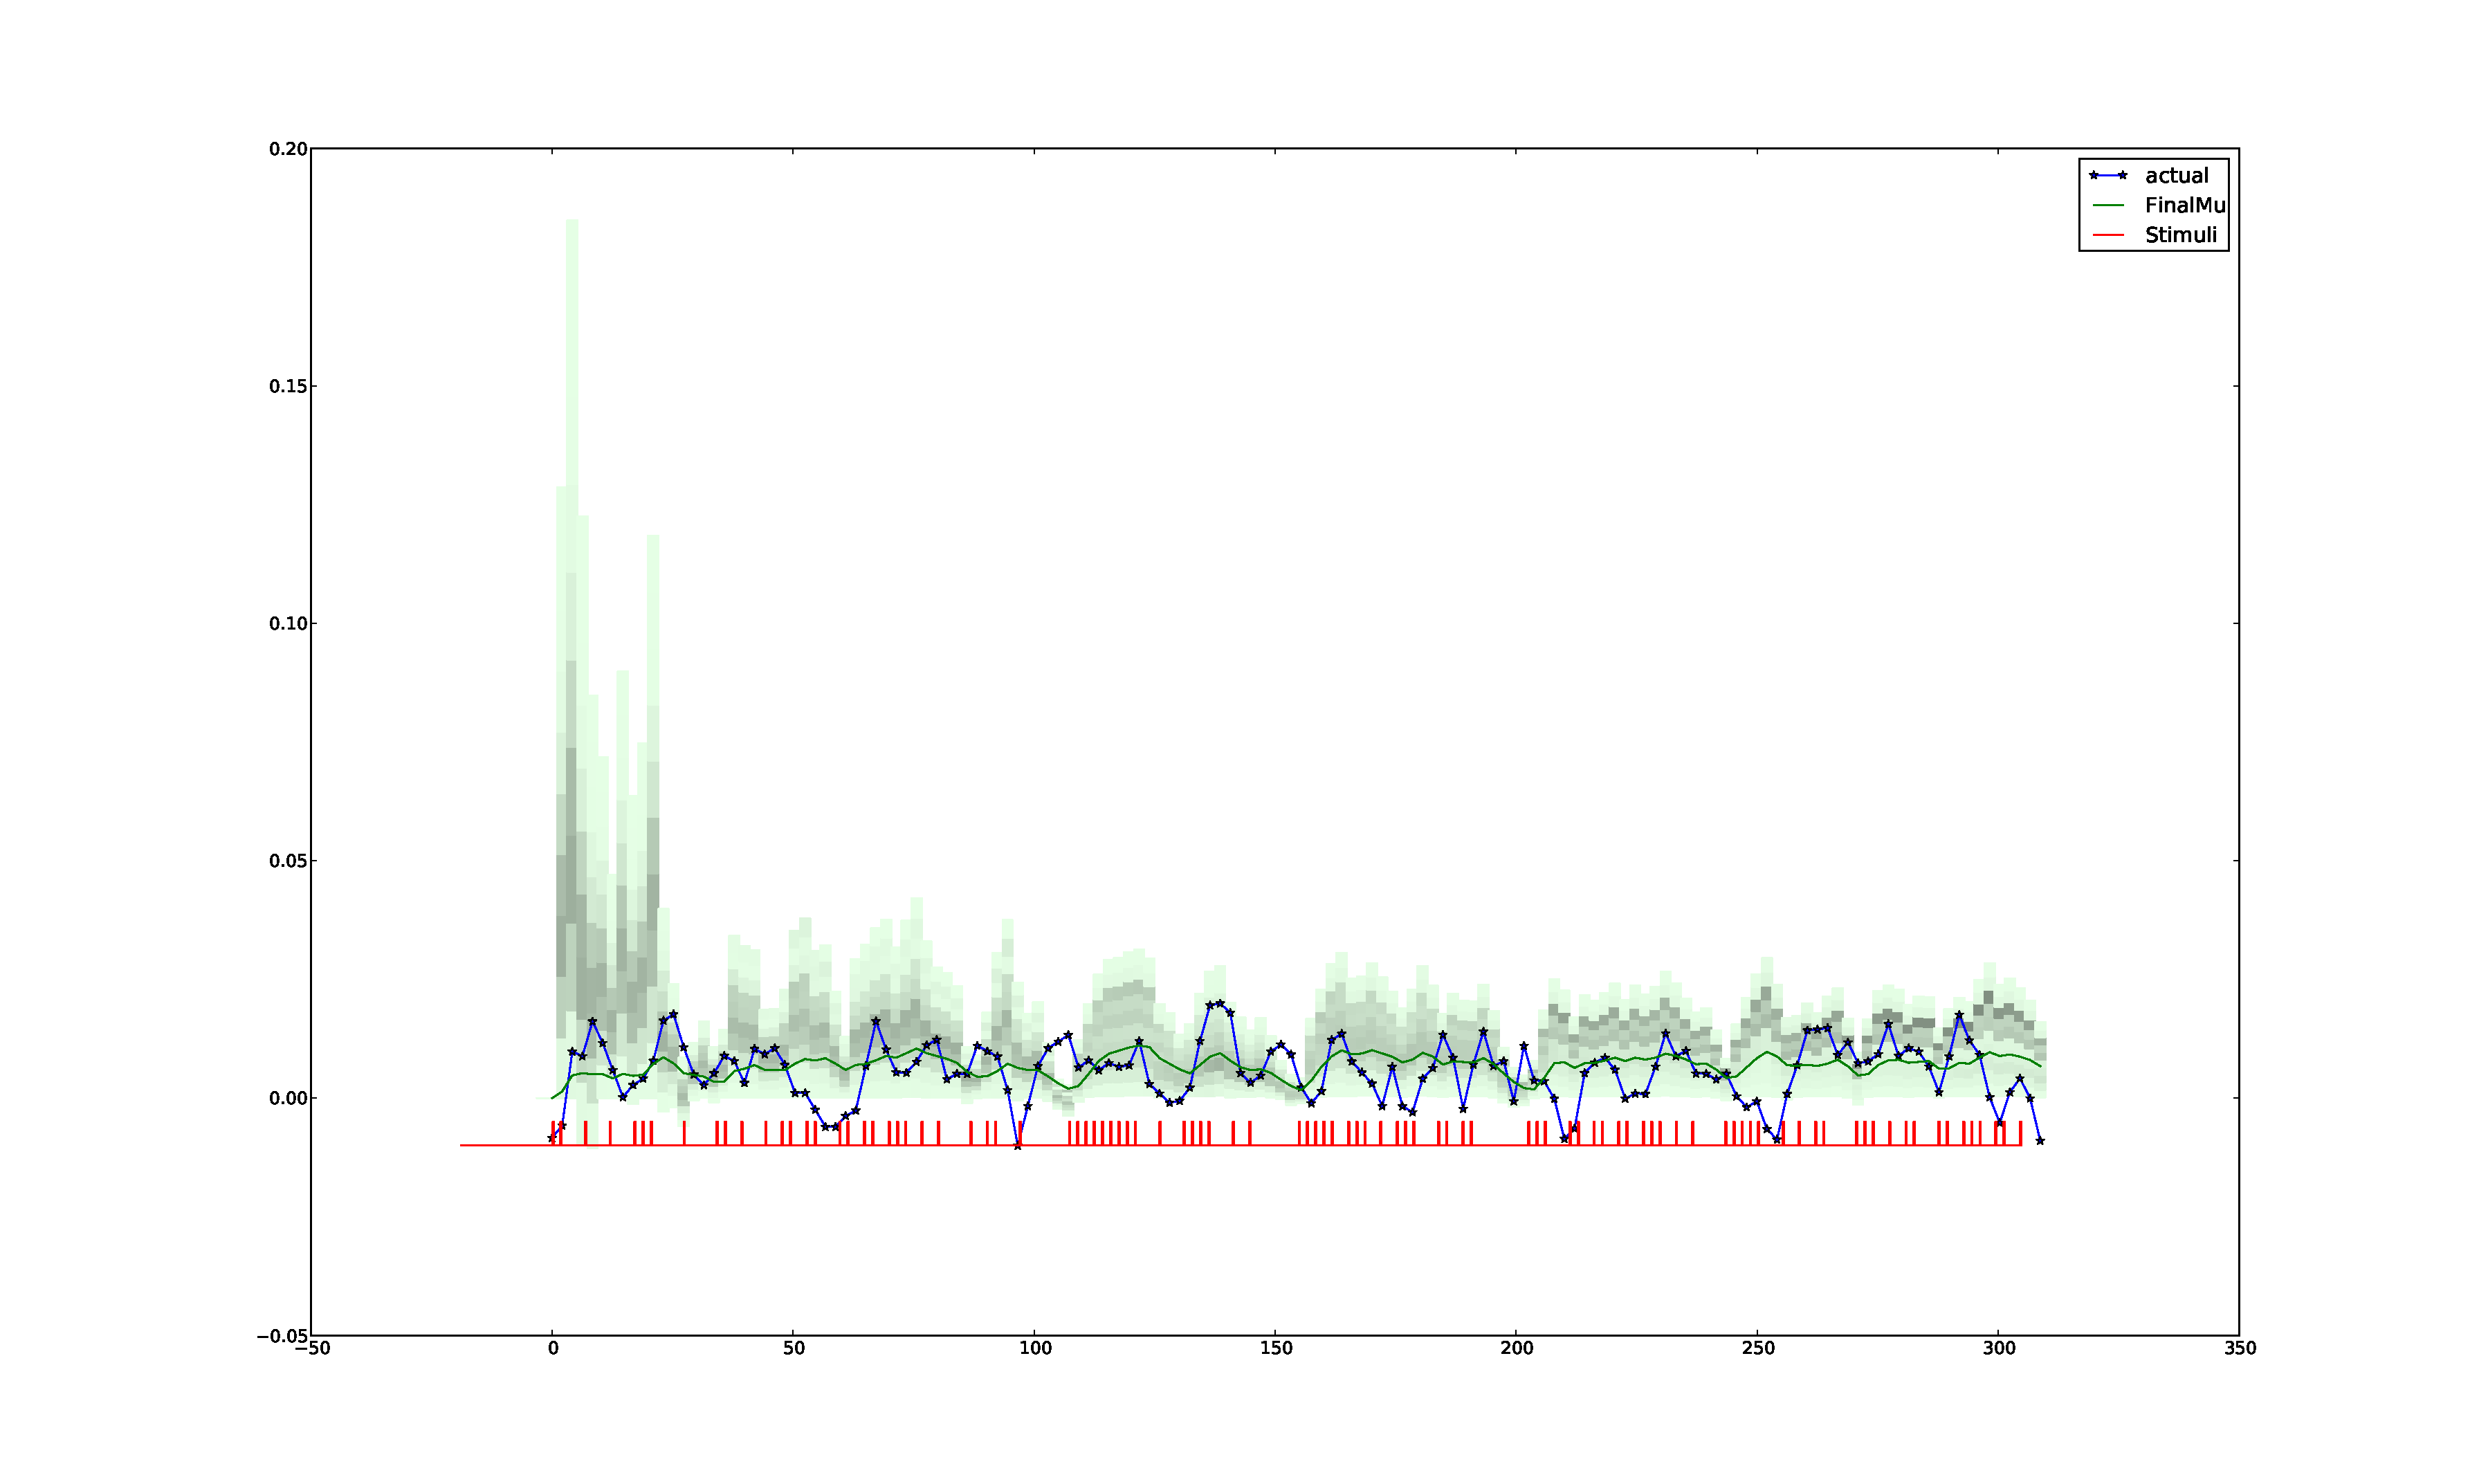
\includegraphics[clip=true,trim=6cm 2cm 6cm 3.5cm,width=7cm]{images/badfit_param1}
\caption{Large variance in time constants over-smoothing.}
\label{fig:badfit_param1}
\end{figure}
In \autoref{fig:badfit_param1}, the particle filter still had not fully converged, and
given more measurements it could still converge to a better estimate. Thus, increases
in the prior variance necessarily must be accompanied by more measurements,
although re-presenting data could be used to artificially extend the measurements. 

\subsection{Detrending}
A large number of de-trending methods were tested, but all had some major problem. 
One viable method that could be utilized given the right experimental design is detrending
based on areas of low activity. This has the advantage that it wouldn't require an arbitrary
constant to be added to the pre-processed signal for the BOLD model to fit properly.
The disadvantage of this approach is that it could hide long fall times by normalizing them
out. It also requires periodic breaks in the stimulus, which could reduce value of those
samples for fitting purposes. 

Another potential way to deal with detrending is to 
linearize. This would use the delta between measurements for fitting rather than the 
direct value. This has the advantage of not requiring detrending and thus 
gives nearly raw data to the particle filter
for processing. The effectiveness of this method depends directly on the type of stimulus.
In an event driven stimulus with sparse stimuli this could be extremely effective because
the DC level has minimal data; however the longer high levels are held the less effective
this will be. On the other hand, splines will also reduce the plateaus, so its possible
linearizing may be just as effective. I found in tests that large drift-low white noise
type signals performed much better with a linearization approach, as one might expect. 
The results were equal to or worse in real data; but that was only for one particular
stimulus sequence. 

A subtle difference that could be made in detrending is how the percent difference
is calculated. In this work the spline was subtracted, and then the result
was divided by the average of the initial signal. A more correct method may be dividing
by the spline value at that particular point. The reason for not dividing by the spline
at that point is that it could be less stable, and in a sense the trend has already
been removed. The difference is not particularly large though 
(dividing by 1020 rather than 1000 for instance) as long as the spline didn't have heavy swings. 

Finally, rather than adding a constant to the detrended data before
applying the particle filter, a DC gain parameter could be added to the model. In
tests, this could work well, however, it often did not. The problem with this
could simply be the addition of another degree of freedom without any increase in
the number of particles. Increasing the number of particles further though
can be computationally intractable. Thus, while this is in a sense the correct
solution, it is an impractical one. 

\subsection{Experimental Changes}
\label{sec:Sideways Measurements}
One definite way of improving the results of the particle filter is more 
measurements. While increasing the sample rate of FMRI scanners may
not be possible, simultaneous measurements of volume and flow is
possible \cite{Hu2009}, albeit at 9T in a cat. Just one of those measurements
though would be extremely powerful when incorporated into the BOLD
model. By adding another measurement, especially for one of the other state
variables (like blood volume and blood flow), the
variance in the parameter estimates would certainly drop. Of course, more measurements
may be gained by simply performing longer FMRI tests, or concatenating several 
together. Even more basic, its possible to artificially increase the number of 
measurements by presenting them the time-series several times. 
This activity is similar to the process used in neural networks,
and gives the particle filter longer to converge to the optimal estimate. On the 
downside, this increases runtime and artificially reduces variance. 
Thus it does not necessarily improve the results. In tests, it did reduce the
final covariance but did not lead to better estimates. 

Additionally, given the non-linearities in the system, differences in stimuli
can make a huge difference in the observability of parameters. The mentality 
for using a physiologically based nonlinear model for BOLD signal is to model 
those nonlinearities. Its logical then that nonlinear parameters may not
be identifiable when the input is primarily an impulse response. Therefore,
a wide range of inputs may shed further light on the parameters than found 
in this work.

As discussed in \autoref{sec:Methods Weighting Function}, choosing a weighting
function is difficult. Automatically estimating measurement error could improve
the quality of the particle filter results. Although I made some attempts to do
this, finding a generic, consistent solution is complex, and often depends on the
experimental design. This problem strikes at the very of heart of the difficulty
in analyzing FMRI, and so it is not likely to be solved soon. 

% Future works
%% Using s as the input to other regions. 
%% Comparison of posterior of parameters
\section{Applications}
There are a number of advantages to the particle filter approach presented
here. In the past FMRI data has been analyzed strictly for determining
correlation between a stimulus and response. With this new method
the correlation is simply a means to determining the joint posterior distribution
of the parameters. While only regions that correlate with the input will 
be calculable, this method exploits that correlation to constrain the 
prior distribution of the parameters. The resulting distribution, while difficult 
to visualize because of the high-dimensionality, could nevertheless be 
correlated with neural pathologies. Despite the fact that the parameters
are under-determined, the final distribution is still a reduction in the
uncertainty of the parameters. This reduction in uncertainty naturally
contains information which may be exploited based on non-parametric 
statistical analyses. 

Because of the limitations present in every image modality in neuroimaging,
its becoming increasingly clear that combining data from multiple sources
will be necessary to push neurology forward. In order to do so however, the
output of each source needs to fully represent what information that source
can provide. Combining the sources using Bayesian statistics is promising
yet often difficult because full probability distributions are hard to come by.
However, in this case, the particle filter provides a full posterior which
is extremely versatile. Therefore, future works will easily be able to
plug in data from multiple sources if they all output Bayesian posteriors.
For instance, if two different modalities have calculated the probability
distribution of neural efficiency, those two beliefs may be combined into
one conditional belief for the probability of neural efficiency. 

An advantageous aspect of using a physiological model such as this, is that
it permits estimates of otherwise hidden parameters. In particular the BOLD
model gives an estimate of the value of the flow inducing signal, $s$. Having
this value available opens up new avenues for determining inter-regional
dependencies. All the regions for which the value of $s$ are trustworthy
correlate closely with the original stimuli, so determining the connection
between their values of $s$ would be less than edifying. Instead, the values
of $s$, which in some sense is the activation in a particular region, could
be used to drive other inputs. Thus, the particle filter could be re-run
with the time-series of a particular voxel's $s$ value as an additional stimulus.
In this way, it could be possible to determine chains of events. This is just
one possible benefit being able to determine the time course of the hidden
state variables present in the BOLD equations; the potential benefits of being
able to determine this information is limitless. Of course, improving the quality
of the parameter estimates is necessary if such information is to be fully
trusted. 


